\documentclass{article}
\usepackage[utf8]{inputenc}

\usepackage{amsfonts}
\usepackage{amssymb}
\usepackage{amsmath}
\usepackage{amsthm}
\usepackage{enumitem}

\usepackage{graphicx}
\usepackage{bbold}
\usepackage{float}
\usepackage{bm}
\usepackage{color}
\usepackage{hyperref}
\usepackage[margin=2.5cm]{geometry}

\usepackage{fancyhdr}

\usepackage[french]{babel}
\usepackage[T1]{fontenc}

\usepackage{tcolorbox}
\usepackage{fancyvrb}
\usepackage{scrextend}

\makeatletter

\makeatother

\begin{document}

% ==============================================================================

\title{Projet Geurts 2022}								% Title
\author{Maxime FIRRINCIELI, Romain LAMBERMONT, Arthur LOUIS}								% Author
\date{\today}											% Date

\makeatletter
\let\thetitle\@title
\let\theauthor\@author
\let\thedate\@date
\makeatother

\pagestyle{fancy}
\fancyhf{}
\rhead{\theauthor}
\lhead{\thetitle}
\cfoot{\thepage}

\begin{titlepage}
 \centering
 \vspace*{0.5 cm}
 
\includegraphics[scale = 0.7]{figs/facsa.png}\\[1.0 cm]	% University Logo
 \textsc{\LARGE \newline\newline Faculté des Sciences appliquées}\\[2.0 cm]	% University Name
 \textsc{\Large MATH0488-1 Éléments de Processus Stochastiques}\\[0.5 cm]				% Course Code
 \rule{\linewidth}{0.2 mm} \\[0.4 cm]
 {\huge \bfseries Méthodes de Monte Carlo par chaînes de Markov pour la détection de communautés dans un graphe}\\
 \rule{\linewidth}{0.2 mm} \\[1.5 cm]

 \begin{minipage}{0.5\textwidth}
 	\begin{flushleft} \large
 		\emph{Professeur :}\\
 		  Pierre GEURTS\\
    \vspace{0.5cm}
 		\end{flushleft}
 		\end{minipage}~
 		\begin{minipage}{0.4\textwidth}

 		\begin{flushright} \large
 		\emph{Groupe :} \\
      Maxime FIRRINCIELI\\
      Romain LAMBERMONT\\
      Arthur LOUIS\\
 	\end{flushright}

 \end{minipage}\\[2 cm]


 \thedate
\end{titlepage}

% ==============================================================================
\thispagestyle{empty}
\tableofcontents
\listoffigures
\listoftables
\pagebreak
\setcounter{page}{1}

\section*{Introduction}
Ce projet a pour but de détecter les communautés dans un graphe grâce aux chaînes de Markov et par les méthodes de Monte-Carlo. L'utilisation de ces outils nous permettra de détecter efficacement les communautés dans un graphe.
Le projet sera constitué en deux parties. Une première se focalisera sur la familiarisation avec les chaînes de Markov et les méthodes de Monte-Carlo, plus précisement l'algorithme de Metropolis-Hastings, tandis que la seconde sera le cœur du projet 
avec la recherche de communautés dans un graphe.

\section{Première partie : chaînes de Markov et algorithme MCMC}

\subsection{Chaînes de Markov}
\paragraph{}
Rappelons d'abord brievement ce qu'est une chaîne de Markov. Une chaîne de Markov est un outil mathématique stochastique, qui utilise un principe de "non-mémoire". Tout état d'un système est simplement calculé à partir du précédent, ce qui en facilite l'analyse.
\\\\
Ces chaînes sont simplement décrites mathématiquement comme suit avec $X_1, X_2,..., X_t$ une suite de variables aléatoires qui définit une chaîne de Markov
si (pour t > 1) elle suit cette relation :
\begin{equation*}
  \mathbb{P}(X_1, X_2, ..., X_t) = \mathbb{P}(X_1)\prod_{l = 2}^{t}\mathbb{P}(X_l | X_{l-1}) 
\end{equation*}

\subsubsection{}

Nous calculons donc pour des valeurs de $t$ croissantes les différentes valeurs demandées, ici avec $t = 20$ (suffit pour avoir convergé) :
\begin{itemize}
  \item Cas de base distribué uniformément : $\mathbb{P}(X_t = x) = 
  \begin{pmatrix}
    0.3488 & 0.0698 & 0.2326 & 0.3488\\
  \end{pmatrix}$ avec $x = 1, 2, 3, 4$
  \item Cas de base fixé : $\mathbb{P}(X_t = x) = 
  \begin{pmatrix}
    0.3488 & 0.0698 & 0.2326 & 0.3488\\
  \end{pmatrix}$ avec $x = 1, 2, 3, 4$
  \item $Q^t = 
  \begin{pmatrix}
  0.3488 & 0.0698 & 0.2325 & 0.3488\\
  0.3488 & 0.0698 & 0.2326 & 0.3488\\
  0.3488 & 0.0698 & 0.2326 & 0.3488\\
  0.3488 & 0.0698 & 0.2326 & 0.3488\\
  \end{pmatrix}$ 
\end{itemize}

On remarque donc bien une convergence vers des probabilités et ceci peut importe le cas de départ, on peut montrer cette convergence sur les figures ci-dessous :
\begin{figure}[h!]
  \centering
  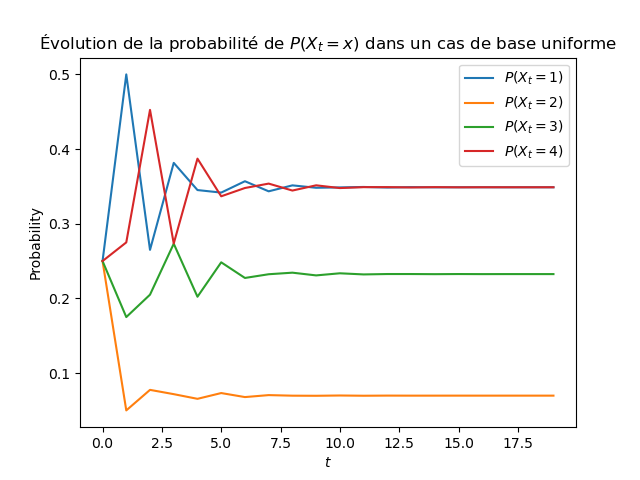
\includegraphics[width=0.5\textwidth]{figs/evo_unif.png}
  \caption{Évolution des probabilités dans une distribution de départ uniforme}
\end{figure}
\\
\begin{figure}[h!]
  \centering
  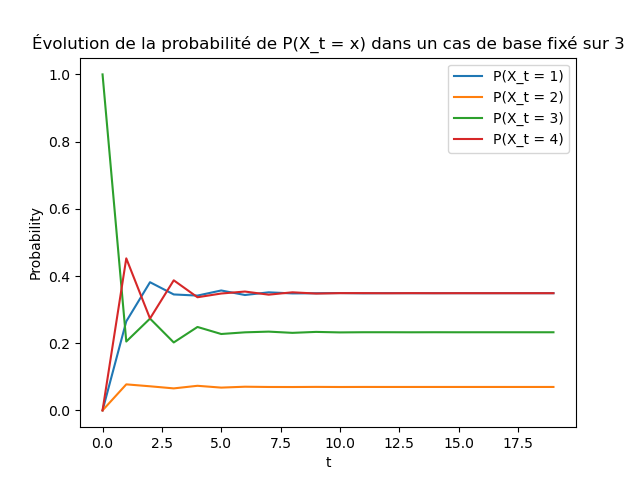
\includegraphics[width=0.5\textwidth]{figs/evo_fixed.png}
  \caption{Évolution des probabilités dans une distribution de départ fixée sur 3}
\end{figure}

\subsubsection{}

Afin de déduire la distribution stationnaire $\pi_{\infty}$ de notre chaîne qui est décrite comme suit :
\begin{equation*}
  [\pi_\infty]_j = \lim_{t \rightarrow \infty} \mathbb{P}(X_t = j)
\end{equation*}

Nous allons simplement calculer $\mathbb{P}(X_t)$ avec un grand $t$ ce qui nous donne :
\begin{equation*}
  \pi_{\infty} = 
  \begin{pmatrix}
    0.3488 & 0.0698 & 0.2326 & 0.3488
  \end{pmatrix}
\end{equation*}

\subsubsection{}
Afin de vérifier les résultats obtenus, nous effectuons des réalisations de notre chaîne de Markov. Nous pouvons mettre en tableau la proportion de réalisation 
de chaque état lors de tests avec un nombre de pas croissant. Nous utilisons un point de départ distribué uniformément entre les 4 états car il a été prouvé
plus haut que ça n'avait pas d'influence.

\begin{table}[h!]
  \begin{tabular}{|c|c|c|c|c|}
  \hline
  \# Pas / État & \multicolumn{1}{c|}{1} & \multicolumn{1}{c|}{2} & \multicolumn{1}{c|}{3} & 4 \\ \hline
  100     & 0.35    & 0.05   & 0.21    & 0.39    \\ \hline
  1000    & 0.351   & 0.075  & 0.23    & 0.344   \\ \hline
  10000   & 0.346   & 0.064  & 0.236   & 0.354   \\ \hline
  100000  & 0.3501  & 0.0722 & 0.228   & 0.3497  \\ \hline
  1000000 & 0.34902 & 0.6757 & 0.23422 & 0.34919 \\ \hline
  \end{tabular}
  \centering
  \caption{Proportion des états obtenus en fonction de nombre de pas}
  \label{tab:table-prop}
\end{table}

En comparant ce tableau avec les résultats obtenus avec les valeurs précédement obtenus, on remarque bien que les proportions sont respectées et font sens, on converge bien 
vers les mêmes valeurs.

\subsubsection{}
/!$\backslash$ TODO /!$\backslash$

\subsection{Méthode MCMC : analyse théorique dans le cas fini}
Nous allons maintenant nous attarder sur l'aspect théorique de l'algorithme de 
Metropolis-Hastings avant de passer à l'aspect pratique.

\subsubsection{}
On veut montrer que $\pi_0$ est une distribution stationnaire sachant que une matrice de transition $Q$ et une distribution initiale $\pi_0$ 
d'une chaîne de Markov invariante dans le temps qui satisfont les équations de balance détaillée :
\begin{equation*}
  \forall i,j \in \{ 1,\dots,N \}, \pi_0(i)[Q]_{i,j} = \pi_0(j)[Q]_{j,i}
\end{equation*}

On reprend donc les définitions de $\pi_0$ et de $Q$ :
\begin{equation*}
  \pi_0 = [P(X_0=x_1) \dots P(X_0=x_k) \dots P(X_0=x_n)]
\end{equation*}
$$Q = \begin{pmatrix}
  P(X_1 = x_1|X_0=x_1) & \dots & P(X_1 = x_n|X_0=x_1)\\
  \dots & P(X_1 = x_n|X_0=x_n) & \dots\\
  P(X_1 = x_1|X_0=x_n) & \dots & P(X_1 = x_n|X_0=x_n)
\end{pmatrix}$$

Sachant que la chaîne de Markov est invariante, on a $Q_0 = Q_1 = \dots = Q_n = Q$ et on sait que la matrice de transition et la distribution initiale respectent les équations de balance détaillée :

\begin{align*}
  \forall i,j \in \{ 1,\dots,N \}, \pi_0(i)[Q]_{i,j} &= \pi_0(j)[Q]_{j,i}\\
  P(X_0=x_i)P(X_1=x_j|X_0=x_i) &= P(X_0 = x_j)P(X_1=x_i|X_0=X_j)\\
  P(X_0=x_i)\frac{P(X_1=x_j,X_0=x_i)}{P(X_0=x_i)} &= P(X_0=x_j)\frac{P(X_1=x_i,X_0=x_j)}{P(X_0=x_j)} \text{ par Bayes}\\
  P(X_1=x_j,X_0=x_i) &= P(X_1=x_i,X_0=x_j) \forall i,j
\end{align*}

On sait également que au vu de la forme de $\pi_0$ et $Q$ vue plus haut et que $\pi_1 = \pi_0 * Q$ :

\begin{align*}
  P(X_1=x_j) &= \sum_{k=1}^n P(X_0=x_k)P(X_1=x_j|X_0=x_k)\\
  P(X_1=x_j) &= \sum_{k=1}^n P(X_0=x_k)\frac{P(X_1=x_j,X_0=x_k)}{P(X_0=x_k)}\\
  P(X_1=x_j) &= \sum_{k=1}^n P(X_1=x_j,X_0=x_k) = \sum_{k=1}^n P(X_1=x_k,X_0=x_j)\\
  P(X_1=x_j) &= \sum_{k=1}^n P(X_1=x_k,X_0=x_j) = P(X_0=x_j)
\end{align*}

On vérifie cela pour chaque $j$, ce qui montre que $\pi_0 = \pi_1$ et que $\pi_0$ est une distribution stationnaire. Cette distribution est unique si la chaîne de Markov induite par la matrice de transition $Q$ est irréductible. 

\subsubsection{}
En remplaçant $p_X$ par $f(x) = cp_X$, on recalcule la probabilté d'acceptation de l'algorithme de Metropolis-Hastings comme suit :

\begin{equation*}
  \alpha(y_{t+1},x_t) = \text{min}(1,\frac{cp_X(y_{t+1})}{cp_X(x_t)}\frac{q(x_t|y_{t+1})}{q(y_{t+1}|x_t)})
\end{equation*}

On peut denoter deux cas en renomant le deuxième membre du min en $\delta$ : 

\begin{itemize}
  \item $\delta < 1$ : On obtient 
  \begin{equation*}
    \alpha(y_{t+1},x_t) = \delta\\
    \alpha(x_t,y_{t+1}) = \text{min}(1,\frac{1}{\delta}) = 1
  \end{equation*}
  \item $\delta > 1$ : On obtient
  \begin{equation*}
    \alpha(y_{t+1},x_t) = 1\\
    \alpha(x_t,y_{t+1}) = \delta
  \end{equation*}
\end{itemize}

Peu importe le cas dans lequel on se trouve, on peut réécrire :
\begin{equation*}
  p_X(x_t)\alpha(y_{t+1},x_t)q(y_{t+1}|x_t) = p_X(y_{t+1})\alpha(x_t,y_{t+1})q(x_t|y_{t+1})
\end{equation*}

On sait que $q(y_{t+1}|x_t)$ 

\begin{equation*}
  p_X(x_t)Q(x_t,y_{t+1}) = p_X(y_{t+1})Q(y_{t+1},x_t)
\end{equation*}

Cette dernière équation est l'équation de balance détaillée et est vérifiée par notre chaîne de Markov.

\subsection{Méthode MCMC : illustration sur un exemple simple}
Nous allons maintenant nous attarder à un cas plus précis de l'algorithme de Metropolis-Hastings pour échantilloner des valeurs suivant la 
distribution binomiale définie comme suit avec $p$ la probabilité de succès :
\begin{equation*}
  \mathbb{P}(X = k) = C_K^k p^k(1-p)^{K-k}
\end{equation*}
Pour ce faire nous allons utiliser la distribution de proposition énoncée avec \(r \in \left] 0, 1\right[\) comme suit :
\begin{equation*}
  q(y|x) = 
  \begin{cases}
    \hfil r & \text{si } x = 0 \text{ et } y = 0\\
    \hfil (1-r) &  \text{si } x = K \text{ et } y = K\\
    \hfil r & \text{si } 0 < x \leq K \text{ et } y = x - 1\\
    \hfil (1-r) & \text{si } 0 \leq x < K \text{ et } y = x + 1\\
    \hfil 0 & \text{sinon}
  \end{cases}
\end{equation*}

\subsubsection{}
Au vu du choix de notre distribution $q(y|x)$ qui est symétrique, on sait que lors du calcul de 
\begin{equation*}
  \frac{p_X(y^{(t)})}{p_X(x^{(t-1)})} \frac{q(x^{(t-1)}|y^{(t)})}{q(y^{(t)}|x^{(t-1)})}
\end{equation*}

La deuxième partie de ce produit se simplifiera au vu de la symétrie de la distribution car
\begin{equation*}
  q(x^{(t-1)}|y^{(t)}) = q(y^{(t)}|x^{(t-1)})
\end{equation*}
On conclut donc que $q(y|x)$ est un bon choix de distribution pour notre algorithme de Metropolis-Hastings comme vu au point 1.2.2 .

\subsubsection{}
Nous allons maintenant réaliser une grande réalisation de notre chaîne de Markov afin de constater la présence d'une convergence :

\begin{figure}[H]
  \centering
  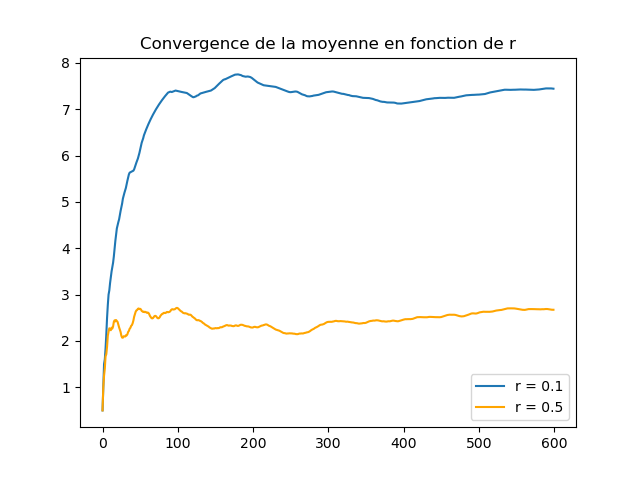
\includegraphics[width=0.5\textwidth]{figs/convergence_mean.png}
  \caption{Convergence de la moyenne pour deux valeurs de $r$}
\end{figure}

\begin{figure}[H]
  \centering
  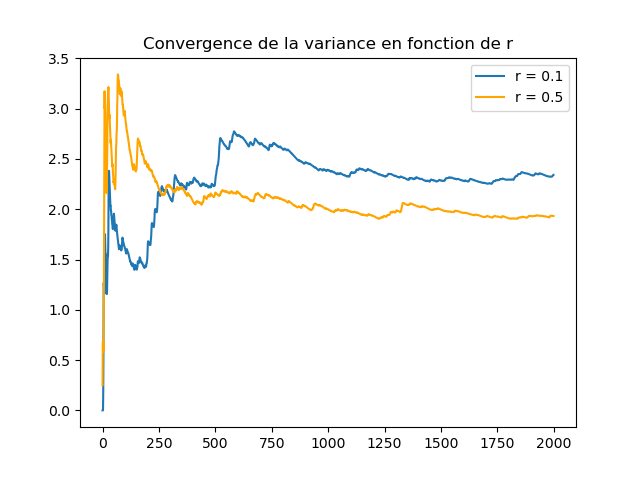
\includegraphics[width=0.5\textwidth]{figs/convergence_var.png}
  \caption{Convergence de la variance pour deux valeurs de $r$}
\end{figure}

Au vu des deux figures ci-dessus, on remarque bien que les valeurs convergent et à des taux différents en fonction de $r$. En effet, plus $r$ est grand, plus on converge rapidement et ce car 
plus $r$ grandit, plus la proportion du cas $0 \leq x \leq K \text{et } y = x-1$ va prendre de l'importance dans notre distribution. Ce qui provoquera une convergence 

\subsubsection{}

\section{Deuxième partie : détection de communautés dans un graphe par algorithmes MCMC}

\subsection{Etude théorique}
\subsubsection{Théorème de bayes, cas général}
\paragraph{}
Pour commencer, rappelons nous le théorème de Bayes dans sa forme général:
\begin{equation*}
    \mathbb{P}(x|y) = \frac{\mathbb{P}(y|x)*\mathbb{P}(x)}{\mathbb{P}(y)}
\end{equation*}
Dans le cadre de ce projet, nous obtenons :
\begin{equation*}
    \mathbb{P}(x|G) = \frac{\mathbb{P}(G|x)*\mathbb{P}(x)}{\mathbb{P}(G)}
\end{equation*}
Regardons maintenant de plus près les 3 termes de notre équation, commençons par $\mathbb{P}(x)$:
\begin{align*}
    \mathbb{P}(x) &= \prod_{u=1}^n p_{x_u} \\ 
                  &= \prod_{i=1}^n p_i^{|\Omega_i(x)|}
\end{align*}
Ensuite, pour la probabilité conditionnelle $\mathbb{P}(G|x)$:
\begin{align*}
    \mathbb{P}(G|x) &= \prod_{1 \leq u < v \leq n} W_{x_u,x_v}^{G_{u,v}} (1-W_{x_u,x_v})^{1-G_{u,v}}\\ 
                    &= \prod_{1 \leq i \leq j \leq k} W_{i,j}^{N_{i,j}(x,G)} (1-W_{i,j})^{N_{i,j}^c(x,G)}
\end{align*}
Et pour finir, grâce à la lois des probabilités totales, nous pouvons transformer $\mathbb{P}(G)$: 
\begin{equation*}
    \mathbb{P}(G) = \int_{}^{} \mathbb{P}(G|x) \, \mathrm{d}x
\end{equation*}
En recombinant ces résultats, nous pouvons exprimer $\mathbb{P}(x|G)$:
\begin{equation*}
    \mathbb{P}(x|G) = \frac{\prod_{i=1}^n p_i^{|\Omega_i(x)|} \prod_{1 \leq i \leq j \leq k} W_{i,j}^{N_{i,j}(x,G)} (1-W_{i,j})^{N_{i,j}^c(x,G)}}{ \int\mathbb{P}(G|x) \, \mathrm{d}x}
\end{equation*}
où:
\begin{align*}
    N_{i,j}(x,G)&=\sum_{u<v,x_u=i,x_v=j} \mathbb{1} (G_{uv}=1) \\
    N_{i,j}^c(x,G) &= \sum_{u<v,x_u=i,x_v=j} \mathbb{1} (G_{uv}=0)\\
                   &= |\Omega_i(x)|*|\Omega_j(x)| - N_{i,j}(x,G) \text{  si }i \ne j\\
                   &= \frac{|\Omega_i(x)|*(|\Omega_i(x)|-1)}{2} - N_{i,i}(x,G) \text{  si }i = j
\end{align*}
\paragraph*{}
Dans le cas d'une distribution $SBM(N,K,p,A,B)$, la probabilité $\mathbb{P}(x|G)$ sera simplifiée.
\begin{align*}
    \mathbb{P}(G|x) &= \prod_{1 \leq i \leq j \leq k} A^{N_{i,i}(x,G)} (1-A)^{N_{i,i}^c(x,G)}\text{ si }i=j\\
                    &= \prod_{1 \leq i \leq j \leq k} B^{N_{i,j}(x,G)} (1-B)^{N_{i,j}^c(x,G)}\text{ si }i \ne j
\end{align*}
\subsubsection{}
\paragraph*{}
Le terme qui va devenir un problème si N augmente, est le dénominateur de la fraction finale du point précédent. En effet, la complexité du calcul de l'intégral
est exponentielle par rapport à N. Cependant, il n'est pas nécéssaire de connaitre ce terme car nous souhaitons maximiser $\mathbb{P}(x|G)$ et l'intégrale se 
simplifiera lors du calcul du taux d'acceptation $\alpha$ car elle est indépendante du vecteur $x$ et donc constante au cours des itérations de l'algorithme de 
Metropolis-Hastings.
\subsubsection{}
Pour que Metropolis-Hastings fonctionne au mieux, il faut que la chaine de Markov générée par celui-ci soit ergodique, c'est-à-dire que tout état soit atteignable depuis n'importe quel autre état,
en un nombre fini de pas. (graphe connexe et irréductible) \\
Ici, dans notre distribution $q_{s}$, on vient modifier au hasard une composante à la fois du graphe ce qui nous assure de couvrir toutes les possibilités/états et qui nous assure donc une chaine de Markov ergodique.
\subsubsection{}
Le taux d'acceptation $\alpha$ peut être exprimé:
\begin{align*}
    \alpha &= \frac{\mathbb{P}(x_t|G)}{\mathbb{P}(x_{t-1}|G)} \\
           &=\frac{\frac{\prod_{i=1}^n p_i^{|\Omega_i(x_t)|} \prod_{1 \leq i \leq j \leq k} W_{i,j}^{N_{ij}(x_t,G)} (1-W_{i,j})^{N_{i,j}^c(x_t,G)}}{ \int_{}^{} \mathbb{P}(G|x) \, \mathrm{d}x}}{\frac{\prod_{i=1}^n p_i^{|\Omega_i(x_{t-1})|} \prod_{1 \leq i \leq j \leq k} W_{i,j}^{N_{i,j}(x_{t-1},G)} (1-W_{i,j})^{N_{i,j}^c(x_{t-1},G)}}{ \int\mathbb{P}(G|x) \, \mathrm{d}x}}\\
           &=\frac{\prod_{i=1}^n p_i^{|\Omega_i(x_t)|} \prod_{1 \leq i \leq j \leq k} W_{i,j}^{N_{ij}(x_t,G)} (1-W_{i,j})^{N_{i,j}^c(x_t,G)}}{\prod_{i=1}^n p_i^{|\Omega_i(x_{t-1})|} \prod_{1 \leq i \leq j \leq k} W_{i,j}^{N_{i,j}(x_{t-1},G)} (1-W_{i,j})^{N_{i,j}^c(x_{t-1},G)}}
\end{align*}
Comme le taux $\alpha$ sera calculé numériquement, il est intéressant de calculer son logarithme. 
\begin{align*}
    \log (\mathbb{P}(x|G)) &= \sum_{i=1}^k|\Omega_i(x)|\log(p_i) + \sum_{1\leq i \leq j \leq k} N_{i,j}(x,G) \log(W_{i,j})+N_{i,j}^c(x,G)\log(1-W_{i,j})\\
    \log\alpha =& \log (\mathbb{P}(x_t|G)) - \log (\mathbb{P}(x_{t-1}|G))\\
               =& \sum_{i=1}^k|\Omega_i(x_t)|\log(p_i) + \sum_{1\leq i \leq j \leq k} N_{i,j}(x_t,G) \log(W_{i,j})+N_{i,j}^c(x_t,G)\log(1-W_{i,j})\\
               &- \sum_{i=1}^k|\Omega_i(x_{t-1})|\log(p_i) - \sum_{1\leq i \leq j \leq k} N_{i,j}(x{t-1},G) \log(W_{i,j})+N_{i,j}^c(x{t-1},G)\log(1-W_{i,j})\\
               =& \sum_{i=1}^k(|\Omega_i(x_t)|-|\Omega_i(x_{t-1}))\log(p_i) +\sum_{1\leq i \leq j \leq k} (N_{i,j}(x_t,G)-N_{i,i}(x{t-1},G)) \log(W_{i,j})\\
               &+ \sum_{1\leq i \leq j \leq k}(N_{i,j}^c(x_t,G)-N_{i,j}^c(x_{t-1},G))\log(1-W_{i,j})
\end{align*}
Ce calcul peut encore être simplifié en mettant à jour les nombres $N_{i,j}(x,G)$, $N_{i,j}^c(x,G)$ et $\Omega_i(x)$ à partir des itérations précédentes. \\
Nous l'avons implémenté dans notre algorithme pour améliorer grandement les temps d'éxécution.


\newpage
\subsection{Analyse expérimentale}
\subsubsection{}
\paragraph*{}
Les graphiques qui vont suivre sont tous en rapport avec une distribution
 $SBM(500,2,[0.5,0.5],a/500,b/500)$
\begin{figure}[H]
    \centering
    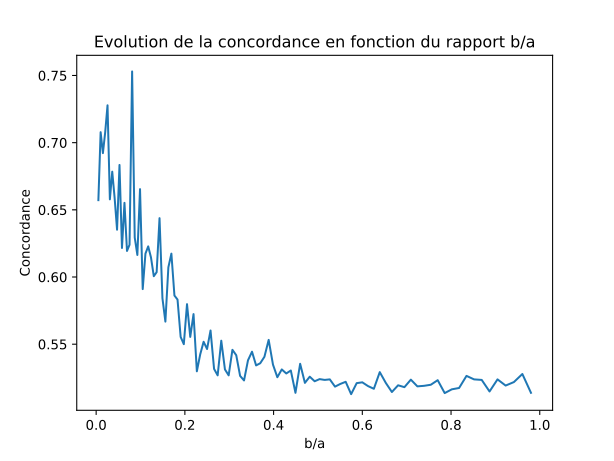
\includegraphics[width=0.5\textwidth]{figs/concordance_a_b.png}
    \caption{Evolution de la concordance en fonction du rapport $b/a$}
\end{figure}
\begin{figure}[H]
    \centering
    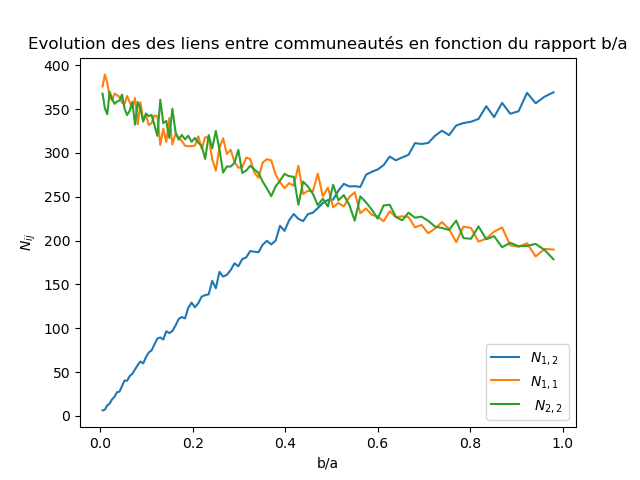
\includegraphics[width=0.5\textwidth]{figs/nij.png}
    \caption{Evolution de la concordance en fonction du rapport $b/a$}
\end{figure}

\paragraph*{}
En comparant les 2 graphiques, on remarque rapidement que moins les communeautes
ont de liens entre elles, plus l'algorithme de Metropolis-Hastings les détecte avec 
précisions. A partir d'un rapport $b/a = 0.2 $ notre algorithme ne donne aucun
résultats concluants

\subsubsection{}

\subsection{Application à un grand graphe}
\subsubsection*{}
\paragraph*{Notre implémentation}
Pour implémenter l'algorithme de Metropolis-Hastings, nous avons décider de 
procéder étape par étape et cela se reflète bien dans nos fonctions. Chaque 
fonction a été une étape dans notre compréhension du problème. \\
Nous avons d'abord créé un générateur de distribution SBM pour bien comprendre les 
rouages de cette distribution. Ensuite, nous avons cherché un moyen de calculer
la probabilité $\mathbb{P}(G)$ avant de nous rendre compte que cela nous serait inutile 
pour notre implémentation. Lorsque nous avons compris ça, nous avons pu avancer.\\
Nous avons poursuivi avec la fonction \textbf{computePX}. Lorsque nous avons simplifié au maximum 
notre problème pour une distribution SBM symétrique, nous nous sommes encore rendu compte
que cette partie était aussi inutile car ce terme reste constant dans notre cas et ne change 
donc rien a la maximisation de $\mathbb{P}(x|G)$. \\
Nous avons donc abordé le dernier morceau qui était en fait le seul utile et 
nous avons rencontrer pas mal de problèmes d'abord du à de simples erreurs de code. \\
Une fois tous ces soucis réglés, nous avions un algorithme fonctionnel mais 
très loin d'être efficace. Nous avons donc fait des analyses temporelles pour trouver la partie 
de notre code qui prenait le plus de temps, c'était la fonction \textbf{computeN}. Nous avons compris
à ce moment la que recalculer à chaque fois tous les éléments $N_{i,j}(x,G)$ n'était pas la bonne 
solution. \\
Nous avons alors implémenté une mise à jour de la variable $N$ à partir de celle du pas
précédent. Il nous a ensuite paru logique d'étendre cette méthode à la variable $Om$. Vous pouvez 
trouver nos étapes de mise à jour des variables dans la fonction \textbf{nextY}. Quand nous avons
passé cette étape, le code à tout de suite été beaucoup plus efficace au point que nous avons doublé
le nombre d'itérations pour atteindre 1.000.000 et cela nous a pris moins de temps que pour la  version précédente.\\
Par après, nous nous sommes demandé comment 
éviter de tomber dans un minimum local et nous avons pensé que faire plusieurs tests en prenant 
différents vecteurs initiaux aléatoires permettrait de prendre en compte la possibilité d'un minimum local.
L'arguments nbTests de notre fonction \textbf{mhALL} est la concrétisation de cette idée.\\
Nous avons alors lancé le test sur le graphe proposé pour le challenge et nous avons obtenus un très 
bon résultat! ($\log(\mathbb{P}(G|x)\mathbb{P}(x)) = -1295577$)
\subsubsection*{Amélioration possible}
\paragraph*{}
Au fil des séances et des heures passées sur ce projet, nous avons compris que nous ne pourrions jamais 
atteindre un résultat parfait et cela pour plusieurs raisons. \\
Premièrement, nous avons des données réelles à analyser. Ces données ne peuvent pas correspondre exactement
à une distribution théorique. \\
Ensuite, nous utilisons une distribution symétrique. En effet, nous avons considéré que la distribution
était uniforme ($p_i = p_j ,\forall i,j \in[1,k]$) et avons posé $W_{i,i}=A$ et $W_{i,j},\forall i,j \in [1,k] ,i \ne j$.
Nous savons cependant que $A = \frac{W_{1,1}+W_{2,2}}{2}$ alors que en pratique, les valeurs sur la diagonale de $W$
sont assez différentes. Nous aurions pu chercher grâce à l'algorithme de Metropolis-Hastings la meilleur combinaison de 
$W_{1,1}$ et $W_{2,2}$ pour avoir une concordance encore plus proche. 
\end{document}